\documentclass[a4paper]{article}

\bibliographystyle{plain}
% algumas packages para arrumar as tables co a margin:
% allows for temporary adjustment of side margins
\usepackage{changepage}
% provides filler text
\usepackage{lipsum}

% just makes the table prettier (see \toprule, \bottomrule, etc. commands below)
\usepackage{booktabs}


\usepackage[brazilian]{babel} %Para traduzir os textos
\usepackage[utf8]{inputenc} %Para poder usar acentos
\usepackage[a4paper]{geometry} %Para ajustar a parte geometrica da folha
\geometry{verbose,tmargin=2cm,bmargin=3cm,lmargin=3cm,rmargin=3cm} %Parte de margens
\setlength{\parindent}{0.5cm}
\usepackage{wrapfig} %Biblioteca Matematica/Grafica
\usepackage{mathptmx} %Biblioteca Matematica/Grafica
\renewcommand{\ttdefault}{mathptmx} %Biblioteca Matematica/Grafica
\usepackage{amsmath} %Biblioteca Matematica/Grafica
\usepackage{amssymb} %Biblioteca Matematica/Grafica
\usepackage[11pt]{moresize}% different letters sizes
\usepackage{float}% enables accurate location of tables
\usepackage{caption}% to make personalized captions
\usepackage{graphicx} %Para inclusão de imagens
\usepackage{indentfirst}
\usepackage{amsfonts}
\usepackage[T1]{fontenc}
\usepackage{fancyref}
%\usepackage[nottoc]{tocbibind}
\usepackage[framed,numbered]{mcode}

\graphicspath{ {images/} }

\makeatletter
\providecommand{\tabularnewline}{\\} %define

\title{Cálculo Computacional do Círculo de Mohr} % main title
\author{EM423 - Resistencia dos Materiais \\ \textsc{Grupo 13}}
\date{22 de Outubro, 2014}

\begin{document} % actually starts the document here
\maketitle

% members of the group
\begin{center}

	\begin{tabular}{l r l}
		Integrantes:\\\\
		 Felipe Tanios & RA: 155330  \\
		 Henrique Noronha Facioli & RA: 157986 \\
		 Kairo Vinicius & RA: 156075 \\
		 Lauro Souza e Cruz & RA: 156175\\
		 Mateus Coelho & RA: 156675 \\
	\end{tabular}
\end{center}


\newpage

\section{Introdução}


A força é uma ação que tende a alterar o estado do corpo,seja em repouso ou em movimento. É possível fazer o corpo acelerar, modificar a velocidade, a direção e o sentido de movimento. 
O estado do corpo submetido à ação de forças em torno de um ponto dentro do corpo material, é chamado de tensão. Força de tensão é uma força que quando aplicada a um corpo elástico, ele tende a se modificar, produzindo uma tensão. A representação desse estado de tensões é chamado de Círculo de Mohr.

Introduzido por  Christian Otto Mohr,  o Círculo de Mohr é uma forma gráfica bidimensional para resolver problemas de momentos de inércia, deformações e estado de tensões baseado na lei de transformação do tensor tensão de Cauchy. É possível usar o Círculo de Mohr somente quando cada plano for representado por um ponto em um sistema de coordenadas ($\sigma,\tau$).

O circulo de Mohr foi muito usado no passado quando não existiam calculadoras eletrônicas para obter graficamente e em escala, respostas para os problemas de distribuição de Tensões, porem atualmente ele é mais usado para visualizar completamente os estados de tensão em um ponto P considerado

\section{Resumo}
Este projeto busca um metodo para o calculo computacional de um círculo de Mohr, assim como uma interface gráfica amigável ao usuario. Para isso foram usadas referencias teóricas fornecidas pelo professor, bem como outras referencias de universidades renomadas. Para a interface foi usada a biblioteca de python TKinter. Assim, foi gerado um programa com interface simples e resultados apresentados ao usuario em uma página html, para facilitar o uso de uma ferramenta tão util, intuitiva e de facil aprendizado.

\section{Objetivo}
Prover uma interface de fácil utilização que, dadas as tensões de cisalhamento e as tensões normais em um plano, exibe em um gráfico personalizado o círculo de Mohr. O programa pode ser executado em múltiplas plataformas (Windows, Linux) e gera um log em formato de página de internet com os dados calculados. 

\section{Metodologia e Resultados}

\subsection{Metodologia}
Inicialmente buscamos um maior conhecimento do circulo de Mohr. Para isso utilizamos o livro texto indicado pelo professor e outro livro também da disciplina. Buscamos tambem outras fontes da propria universidade e bem como de outras universidades renomadas nacionais e internacionais para compreender o funcionamento do circulo e de todas as tensões e angulos apresentados por ele para uma melhor apresentação dos resultados ao usuario final.

Decidimos usar as formulas citadas na  nomear os angulos como vimos nos slides de outros projetos de outros anos da disciplina, fornecidos pelo professor, possíveis de serem vistos na sub-sessão \ref{subsec: Fórmulas}.
Estas imagens tambem podem ser encontradas no capitulo 7 do livro texto que o professor utiliza para a disciplina, além do capitulo 9 de outro livro de Resistencia dos Materiais (R. C. Hibbeler)

Para idealizar nosso software buscamos exemplos já  existentes parecidos como o da universidade PUC-Rio (e-Morh) porem buscamos um ambiente que já estavamos mais acostumados, optando então pela linguagem python e pela biblioteca de interface grafica TkInter. 
Inicialmente começamos com a adaptação de todas as formulas que o circulo de Mohr faz para um codigo em python, visivel na sub-sessão \ref{subsec:Codigo}. Essa linguagem foi escolhida por nós pela boa performance e por ter um codigo visualmente claro, para um melhor entendimento entre os membros do grupo como um todo.

Para o desenvolvimento da interface buscamos além da documentação original da biblioteca e guias em português da Universidade Federal do Rio de Janeiro (UFRJ), projetos com codigo aberto e interface semelhante a que gostariamos. Decidimos que deveriamos tambem colocar uma representação da orientação de cada tensão que o usuario inseriria para o mesmo conseguir utilizar o programa sem grandes duvidas.

Ao final, precisariamos demonstrar ao usuário os resultados finais, já que essa era a função do programa. Para isso vimos que a maioria dos semelhantes apresentavam ou no próprio circulo ou em um documento no formato txt. Decidimos que essas duas opções nao eram tão claras já que um documento no formato txt em alguns sistemas operacionais são abertos em programas pouco intuitivos e no proprio circulo, no nosso caso, dificultaria a compreensão. 

Optamos por, no final, apresentar os resultados em um documento no formato html que é aberto em um navegador de internet, já que quase todos os sistemas operacionais tem um como padrão, logo ao final, o usuario teria uma página de internet apresentando seus resultados de forma bem clara, com todas as variáveis bem descritas como nos exemplos de imagens já citados



\label{subsec: Fórmulas}

	\subsection{Fórmulas e imagens usadas}

		\begin{figure}[!htb]
			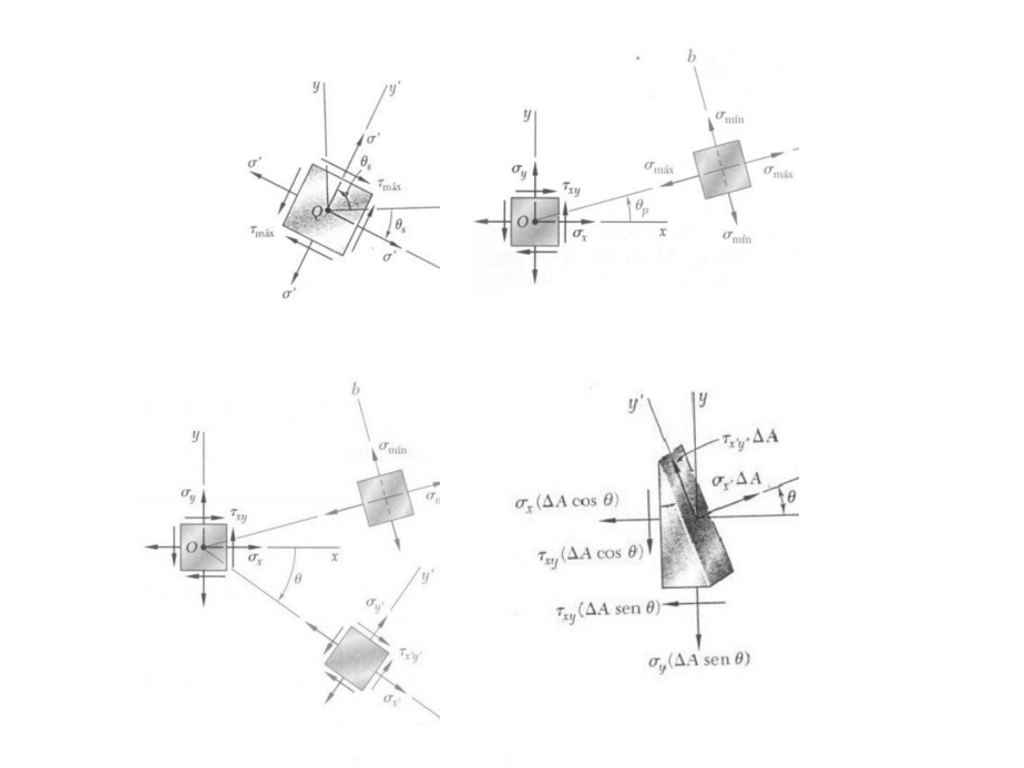
\includegraphics[scale = 0.4]{imagem1}
		\end{figure}	

		\begin{equation}
			\label{sigma_x'}
			\sigma_{x'} = \frac{\sigma_x + \sigma_y}{2} + \frac{\sigma_x - \sigma_y}{2}cos(2 \theta) + \tau_{xy}sen(2\theta)
		\end{equation}

		\begin{equation}
			\label{tau_xy'}	
			\tau_{x'y'} = -\frac{\sigma_x - \sigma_y}{2}sen(2 \theta) + \tau_{xy}cos(2\theta)
		\end{equation}

		\begin{equation}
			\label{sigma_y'}
			\sigma_{y'} = \frac{\sigma_x + \sigma_y}{2} - \frac{\sigma_x - \sigma_y}{2}cos(2 \theta) - \tau_{xy}sen(2\theta)
		\end{equation}

		\begin{equation}
			\sigma_x + \sigma_y = \sigma_{x'} + \sigma_{y'}
		\end{equation}

		\begin{equation}
			(\sigma_{x'} - \frac{\sigma_x + \sigma_y}{2})^2 + \tau_{x'y'}^2 = (\frac{\sigma_x - \sigma_y}{2})^2 + \tau_{xy}^2
		\end{equation}

		\begin{equation}
			\sigma_{med} = \frac{\sigma_x + \sigma_y}{2} 
		\end{equation}

		\begin{equation}
			R =  \sqrt{(\frac{\sigma_x - \sigma_y}{2})^2 + \tau_{xy}^2}  
		\end{equation}

		\begin{equation}
			tg(2\theta_p) = \frac{2\tau_xy}{\sigma_x - \sigma_y}
		\end{equation}

		\begin{equation}
			\sigma_{max} = \sigma{med} + R \therefore \sigma_{max} = \frac{\sigma_x + \sigma_y}{2} + \sqrt{(\frac{\sigma_x - \sigma_y}{2})^2 + \tau_{xy}^2}
		\end{equation}

		\begin{equation}
			\sigma_{max} = \sigma{med} + R
		\end{equation}

		\begin{equation}
			\tau_{max} = \sqrt{(\frac{\sigma_x - \sigma_y}{2})^2 + \tau_{xy}^2}
		\end{equation}

		\begin{equation}
			tg(2\theta_s) = - \frac{\sigma_x - \sigma_y}{2\tau_{xy}}
		\end{equation}

		\begin{equation}
			B = (\sigma_{x'}, \tau_{x'y'})
		\end{equation}

		\begin{equation}
			A = (\sigma_{y'}, -\tau_{x'y'})
		\end{equation} 


\label{subsec: Codigo}

\subsection{Codigo}

\begin{lstlisting}
function run = run(self, tensao_x, tensao_y, tensao_cisalhamento, teta=0)
    sin = math.sin
    cos = math.cos
    rad = math.radians
    tensao_x = tensao_x
    tensao_y = tensao_y
    tensao_cisalhamento = tensao_cisalhamento
    teta = teta
    raio = 0
    % Tensao media (tau_med)
    tensao_principal_med = (tensao_x + tensao_y)/2.

    % Tensao media de Cisalhamento (tau_med)
    tensao_media_cisalhamento = (tensao_x - tensao_y)/2.

    % Raio do Circulo (R)
    raio = ((tensao_media_cisalhamento)**2  + 
                 (tensao_cisalhamento)**2)**0.5

    % Equilibrio das forcas nas direcao do Teta_sigma_x (sigma_x')
    tensao_x_linha = (tensao_principal_med + 
                           tensao_media_cisalhamento*cos(rad(2.*teta)) +
                           tensao_cisalhamento*sin(rad(2*teta)))

    % Equilibrio das forcas na direcao Teta_sigma_y (sigma_y')
    tensao_y_linha = (tensao_principal_med - 
                           tensao_media_cisalhamento*cos(2.*rad(teta)) -
                           tensao_cisalhamento*sin(2.*rad(teta)))

    % Equilibrio das forcas na direcao de Teta_tau (tau')
    tensao_cisalhamento_linha = -s elf.tensao_media_cisalhamento * 
                                        sin(2.*rad(teta))                     
                                        tensao_cisalhamento*cos(2.*rad(teta))

    % Tensao principal maxima (sigma_max)
    tensao_principal_max = tensao_principal_med + 
                                (((tensao_media_cisalhamento)**2) + 
                                tensao_cisalhamento**2)**0.5

    % Tensao principal minima (sigma_min)
    tensao_principal_min = tensao_principal_med - 
                            (((tensao_media_cisalhamento)**2) + 
                                tensao_cisalhamento**2)**0.5

    % Tensao de cisalhamento maxima (tau_max)
    tensao_cisalhamento_max = ((tensao_media_cisalhamento**2) + 
                                        tensao_cisalhamento**2)**0.5

    % Angulo entre os eixos sem rotacao ate o sigma minimo
    teta_p = ((math.degrees(math.atan((2.*tensao_cisalhamento) /
                                          (tensao_x-tensao_y))))/2.)
    % Angulo entre o eixo sem rotacao ate sigma_x'
    teta_s = ((math.degrees(math.atan(-(tensao_x-tensao_y) /
                                          (2.*tensao_cisalhamento))))/2.
\end{lstlisting}

\subsection{Interface}

	\begin{figure}[!htb]
			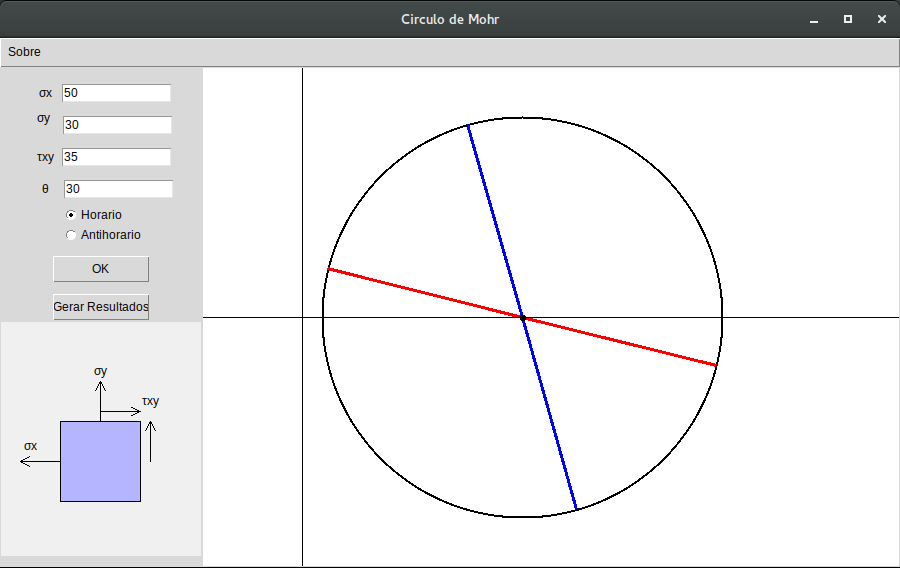
\includegraphics[scale = 0.4]{interfacecirculo}
	\end{figure}	
		
	\begin{figure}[!htb]
		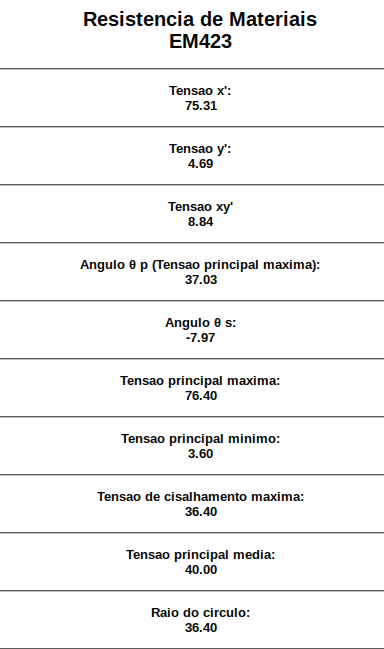
\includegraphics[scale = 0.4]{resultadohtml}
	\end{figure}	


\subsection{Resultados}
Testamos o nosso programa com problemas padrões do livro texto e de listas de exercícios e vimos que o resultado era igual, (em alguns casos com mais casas de precisão numerica). Todos os casos testes tiveram resultados já esperados.

\section{Conclusão}

O círculo de Mohr tem sido empregado há muitos anos para simplificar o cálculo das tensões normais e de cisalhamente em um plano que secciona um corpo qualquer. Este cálculo, por sua vez, é muito importante na área de resistência de materiais, de modo geral, mas tem uma especial atenção principalmente no estudo da deformação de corpos, como metais, e no estudo da mecânica dos solos. Um exemplo da aplicação do cículo de Mohr no estudo dos solos se dá quando é necessário obter a resistência máxima de cisalhamento de um solo. Mais específicamente, segundo o critério de Mohr, há ruptura em um ponto de um solo quando a tensão de cisalhamento é igual à tensão intrínseca de cisalhamento do material, que depende da pressão normal atuante nesse ponto.

Um ponto que deve ser ressaltado para concluir esse projeto é que o círculo de Mohr, apesar de como citado anteriormente ser usado por muitos anos, na atualidade encontra-se desatualizado e pouco utilizado por causa do avanço computacional, o qual diminuiu consideravelmente a velocidade e o tempo gasto para fazer contas simples como as citadas durante todo esse projeto. Entretanto, ainda é muito importante no ensino pois é uma técnica didática e de fácil entendimento de decompor tensões em planos.

\section{Bibliografia}

HIBBELER, R.C., Resistência dos Materiais, Quinta Edição, Pearson, 2004.

BEER, F. P.; JOHNSTON E. R. Resistência dos Materiais. 2. Ed. São Paulo: McGraw Hill,1982.

LAGACE, P. A., Unified Handout Materials And Structures, disponível em $http://web.mit.edu/16.unified/www/FALL/materials/documents/HO-M-6(Mohrs)(08).pdf$, Acesso em 29 de Outubro de 2015

A. P. Santos, E. O. Schaden, P. G. Rubira, T. J. Silva, O Círculo de Mohr, disponível em: $http://www.fem.unicamp.br/~assump/Projetos/2010/g9.pdf$, Acesso em 12 de Novembro de 2015

Python Community, TkInter, disponível em: $https://wiki.python.org/moin/TkInter$, Acesso em 03 de Novembro de 2015.

N. T. Mascia, Teoria das Tensões, disponível em: $http://www.fec.unicamp.br/~nilson/ApostilaTensao.pdf$, Acesso 29 de Outubro de 2015

BRITTO, H., Curso Básico de Resistencia dos Materiais: Fascículo No 9, Estado duplo de tensão. O círculo de Mohr, disponível em: $http://www.lem.ep.usp.br/pef2301/estado_duplo.pdf$, Acesso em 29 de Outubro de 2015

BUFFONI, S. S. O, Transformação de Tensão ou Análise de Tensão, disponível em: $http://www.professores.uff.br/salete/res1/aula61.pdf$, Acesso em 29 de Outubro de 2015

LABAKI, J. Introdução a Python, Modulo C: TKinter, disponível em: $http://www.dcc.ufrj.br/~fabiom/mab225/tutorialtkinter.pdf$, Acesso em 03 de Novembro

MARTHA, L. F.; CARBONO, A. J.; PEREIRA, A. R.; RAMIRES, F. B.; DALCANAL, P. R.; ARAUJO, R. R.; disponível em: $http://webserver2.tecgraf.puc-rio.br/etools/mohr/$, Acesso em 15 de Outubro de 2015


\end{document}
